\documentclass[tikz]{standalone}
\usepackage{mathpazo}

\begin{document}

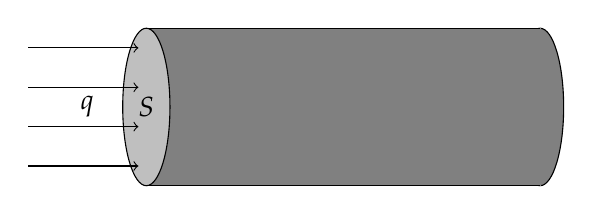
\begin{tikzpicture}
\draw[draw=black, fill=gray] (5,0) ellipse (.3 and 1);
\draw[draw=gray,fill=gray] (0,1) rectangle (5,-1);
\draw (0,-1) -- (5,-1);
\draw (0,1) -- (5,1);
\draw[draw=black, fill=gray!50] (0,0) ellipse (.3 and 1);
\draw (0,0) node {$S$};
\draw[->] (-1.5,.75) -- (-.1, .75);
\draw[->] (-1.5,.25) -- (-.1, .25);
\draw[->] (-1.5,-.25) -- (-.1, -.25);
\draw[->] (-1.5,-.75) -- (-.1, -.75);
\draw (-.75, 0) node {$q$};
\end{tikzpicture}
\end{document}